\documentclass[11pt]{charter}

% El títulos de la memoria, se usa en la carátula y se puede usar el cualquier lugar del documento con el comando \ttitle
\titulo{Detección de lesiones óseas por medio de bioimpedancia: pruebas clínicas y portabilidad} 

% Nombre del posgrado, se usa en la carátula y se puede usar el cualquier lugar del documento con el comando \degreename
\posgrado{Carrera de Especialización en Sistemas Embebidos} 
%\posgrado{Carrera de Especialización en Internet de las Cosas} 
%\posgrado{Carrera de Especialización en Intelegencia Artificial}
%\posgrado{Maestría en Sistemas Embebidos} 
%\posgrado{Maestría en Internet de las cosas}

% Tu nombre, se puede usar el cualquier lugar del documento con el comando \authorname
\autor{Antonio H. Dell'Osa} 

% El nombre del director y co-director, se puede usar el cualquier lugar del documento con el comando \supname y \cosupname y \pertesupname y \pertecosupname
\director{Antonio H. Dell'Osa}
\pertenenciaDirector{IDEI/UNTDF} 
% FIXME:NO IMPLEMENTADO EL CODIRECTOR ni su pertenencia
\codirector{} % si queda vacio no se deberíá incluir 
\pertenenciaCoDirector{}

% Nombre del cliente, quien va a aprobar los resultados del proyecto, se puede usar con el comando \clientename y \empclientename
\cliente{Dr. Fernando Santiago}
\empresaCliente{Universidad Nacional de Tierra del Fuego}

% Nombre y pertenencia de los jurados, se pueden usar el cualquier lugar del documento con el comando \jurunoname, \jurdosname y \jurtresname y \perteunoname, \pertedosname y \pertetresname.
\juradoUno{Determinado por la SCyT-UNTDF}
\pertenenciaJurUno{Evaluador anónimo} 
\juradoDos{Evaluador anónimo}
\pertenenciaJurDos{Determinado por la SCyT-UNTDF}
\juradoTres{Evaluador anónimo}
\pertenenciaJurTres{Determinado por la SCyT-UNTDF}
 
\fechaINICIO{22 de junio de 2020}		%Fecha de inicio de la cursada de GdP \fechaInicioName
\fechaFINALPlanificacion{22 de Agosto de 2020} 	%Fecha de final de cursada de GdP
\fechaFINALTrabajo{04 de diciembre de 2020}		%Fecha de defensa pública del trabajo final


\begin{document}

\maketitle
\thispagestyle{empty}
\pagebreak


\thispagestyle{empty}
{\setlength{\parskip}{0pt}
\tableofcontents{}
}
\pagebreak


\section{Registros de cambios}
\label{sec:registro}


\begin{table}[ht]
\label{tab:registro}
\centering

\begin{tabularx}{\linewidth}{@{}|c|X|c|@{}}
\hline
\rowcolor[HTML]{C0C0C0} 
Revisión & \multicolumn{1}{c|}{\cellcolor[HTML]{C0C0C0}Detalles de los cambios realizados} & Fecha      \\ \hline
1.0      & Creación del documento                                                          & 22/06/2020 \\ \hline
1.1.1      & Primera entrega (2 $\rightarrow$ 3) para ser revisada (Faltantes: Requerimientos y WBS) & 10/07/2020 \\ \hline
1.1.2      & Segunda entrega (2 $\rightarrow$ 3) completa para ser revisada  & 17/07/2020 \\ \hline
1.2      & Primera entrega (3 $\rightarrow$ 4) para ser revisada  & 31/07/2020 \\ \hline

\end{tabularx}
\end{table}

\pagebreak


\section{Acta de Constitución del Proyecto}
\label{sec:acta}

\begin{flushright}
Buenos Aires, \fechaInicioName
\end{flushright}

\vspace{2cm}

Por medio de la presente se acuerda con el Ing. \authorname\hspace{1px} que su Trabajo Final de la \degreename\hspace{1px} se titulará ``\ttitle'', consistirá esencialmente en el prototipo preliminar de un analizador multifrecuencia de bioimpedancia portátil para mediciones no invasivas en seres humanos que permita cuantificar la integración ósea de huesos largos en una escala interpretable por el usuario-médico en seres humanos, y tendrá un presupuesto preliminar estimado de 600 hs de trabajo y 90.000,00 pesos argentinos, con fecha de inicio \fechaInicioName\hspace{1px} y fecha de presentación pública \fechaFinalName.

Se adjunta a esta acta la planificación inicial.

\vfill

% Esta parte se construye sola con la información que hayan cargado en el preámbulo del documento y no debe modificarla
\begin{table}[ht]
\centering
\begin{tabular}{ccc}
\begin{tabular}[c]{@{}c@{}}Ariel Lutenberg \\ Director posgrado FIUBA\end{tabular} &  & \begin{tabular}[c]{@{}c@{}}\clientename \\ \empclientename \end{tabular} \vspace{2.5cm} \\ 
\multicolumn{3}{c}{\begin{tabular}[c]{@{}c@{}} \supname \\ Director del Trabajo Final\end{tabular}} \vspace{2.5cm} \\
%\begin{tabular}[c]{@{}c@{}}\jurunoname \\ Jurado del Trabajo Final\end{tabular}     &  & \begin{tabular}[c]{@{}c@{}}\jurdosname\\ Jurado del Trabajo Final\end{tabular}  \vspace{2.5cm}  \\
%\multicolumn{3}{c}{\begin{tabular}[c]{@{}c@{}} \jurtresname\\ Jurado del Trabajo Final\end{tabular}} \vspace{.5cm}                                                                     
\end{tabular}
\end{table}




\section{Descripción técnica-conceptual del Proyecto a realizar}
\label{sec:descripcion}

\begin{consigna}{black}
A partir del descubrimiento de la radiología por emisión de rayos X para la generación de imágenes diagnósticas este campo de la medicina no ha dejado de crecer: ecografía por ultrasonido, tomografía axial computada, angiografía, resonancia magnética, entre otras. No obstante, con ninguna de estas técnicas se ha podido proyectar un equipamiento portátil que permita detectar fracturas de lesiones óseas. 
En este proyecto se propone el desarrollo de un dispositivo portátil para la detección de fracturas de huesos largos por medio del análisis de propiedades eléctricas, es decir, medidas de bioimpedancia. Este tipo de tecnología brinda la posibilidad de ser aplicada en equipos electrónicos portátiles como solución a la atención de emergencias médicas en tres escenarios: lugares de geografías extremas aisladas (zonas de montaña o continente antártico), lugares aislados (lejos de centros de salud) y zonas urbanas (generando un diagnóstico temprano que evite el traslado de un paciente a un centro hospitalario). Esto proveería diagnósticos in-situ, in-vivo, inocuos y no invasivos, lo que constituye a este proyecto en un desarrollo sin antecedentes a nivel mundial.

El Ing. Dell'Osa con colegas externos a este proyecto ha realizado modelos físicos y computacionales para estudiar la variación de las mediciones de bioimpedancia sobre estructuras biológicas con hueso roto y entero y la dispersión de las corrientes eléctricas aplicadas en el tejido humano in-vivo. A su vez, en colaboración con investigadores del Policlínico Universitario de Cagliari (Italia) se elaboró un protocolo para mediciones clínicas sobre pacientes y voluntarios que fue implementado sobre un dispositivo no-portátil basado en el AD5933EB (Analog Devices©, USA) con una interfaz altamente técnica para el usuario-médico.

En el presente proyecto consta del desarrollo de un prototipo preliminar de un analizador multifrecuencia de bioimpedancia portátil para mediciones no invasivas en seres humanos que permita cuantificar la integración ósea de huesos largos en una escala y una intefaz interpretable por el usuario-médico.

En la Figura \ref{fig:diagBloques} se muestra en un diagrama en bloques las partes principales del sistema a desarrollar. El sistema de control, comunicación y grabado de mediciones está implementado por medio de Raspeberry Pi 4 que se comunica por medio de I2C con un sistemas basado en el AD5933 que es el encargado de tomar las mediciones en configuración bipolar. La interfaz con el usuario-médico se brindará por medio de una aplicación para Smartphone, tablet y PC, la comunicación entre este dispositivo y la Raspberry Pi 4 será inalámbrica (WiFi o Bluetooth).

El circuito integrado AD5933 (Analog Devices, USA) tiene en sí mismo implementadas las soluciones necesarias al análisis espectróscopico de impedancia. El sistema basado en este integrado es una de las tareas de este proyecto.

El presente proyecto enmarca la tesis doctoral del Ing. Dell’Osa.

\vspace{25px}

\begin{figure}[H]
\centering 
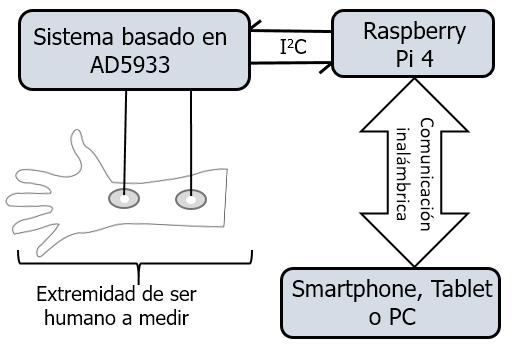
\includegraphics[width=.7\textwidth]{./Figuras/diagBloques_def.png}
\caption{Diagrama en bloques del sistema}
\label{fig:diagBloques}
\end{figure}

\vspace{25px}
\end{consigna}

\pagebreak

\section{Identificación y análisis de los interesados}
\label{sec:interesados}

\begin{consigna}{black} 

\begin{table}[ht]
%\caption{Identificación de los interesados}
%\label{tab:interesados}
\begin{tabularx}{\linewidth}{@{}|X|X|X|X|@{}}
\hline
\rowcolor[HTML]{C0C0C0} 
Rol           & Nombre y Apellido & Organización 	& Puesto 	\\ \hline
Auspiciante y cliente  & \clientename      &\empclientename	& Secretario de Ciencia y Tecnología \\ \hline
Responsable   & \authorname       & \empclientename	& Director 	\\ \hline
Colaboradores & Ing. Agustín Mailing \newline \newline Lic. Fernando Silva \newline Dr.Alejandro Masner &              Independiente-FIUBA \newline Independiente \newline Universidad de la República (Uruguay)	& - \newline \newline Ref: Clínico \newline - 	\\ \hline
Equipo        & Dr. Diego Dondo \newline Lic. Guillermo Prisching & FRC-UTN \newline \empclientename & Ref: Electrónica \newline Ref: Software \\ \hline
\end{tabularx}
\end{table}






\begin{itemize}
\item Auspiciante y cliente: está condicionado por la situación presupuestaria de la Universidad a causa de la actual pandemia que condiciona la economía Nacional. La rendición de gastos se rige por la Ordenanda 5 del Consejo Superior de la \empclientename. Se cuenta con él y el trabajo de la directora de Ciencia y Tecnología y encargo de la Unidad de Vinculación Tecnológica. La rendición final del proyecto será evaluada sólo por el informe final que se debe presentar y la consecuente rendición de gastos.
\item Equipo: Diego Dondo tiene actividad docente durante los dos cuatrimestres y su disponibilidad puede condicionarse temporalmente por sus laborales en su universidad de origen. Guillermo Prisching es su primera interacción con un proyecto con el equipo y colaboradores, a priori, sus referencias hablan de compromiso y responsabilidad.
\item Colaboradores: Agustín Mailing tiene mucho compromiso y disponibilidad pero se encuentra condicionado con su condición de trabajador independiente/autónomo. Fernando Silva es kinesiologo y el aporte clínico del proyecto, puede condicionarse su aporte por el actual contexto de Pandemia y Emergencia Sanitaria.

\end{itemize}

\end{consigna}

\pagebreak

\section{1. Propósito del proyecto}
\label{sec:proposito}

\begin{consigna}{black}
El propósito de este proyecto es el desarrollo de un prototipo calibrado y funcional de un bioimpedanciómetro para el uso específico de detección de fracturas de huesos largos en extremidades; brindando la posibilidad de un diagnóstico in-situ, no invasivo e inocuo para el paciente.
A su vez, permite continuar con expansión de aplicaciones biomédicas basadas en mediciones bioimpedancia en pos de reemplazar (parcial o totalmente) métodos de diagnósticos de fisiopatologías en seres humanos que requieren de tecnologías médica con un alto grado de complejidad tecnológica, adecuación del medio ambiente hostitalario para su utilización y suministro de energía eléctrica de redes de media y/o alta tensión.
Fundándose las razones del desarrollo de este proyecto tanto en la implementación de una nueva técnica diagnóstica con ventajas parciales sobre las existentes y una tecnología médica con un menor impacto al medio ambiente que las actuales.

\end{consigna}

\pagebreak

\section{2. Alcance del proyecto}
\label{sec:alcance}

\begin{consigna}{black}
El presente proyecto incluye el desarrollo de un dispositivo de medición de bioimpedancia en configuración bipolar basado en el integrado AD5933 (Analog Devices, USA) para ser aplicado de modo no invasivo sobre seres humanos. El dispositivo debe ser alimentado a baterías, garantizando su autonomía y portabilidad durante -al menos- 2 horas de uso continuo.

El dispositivo deberá realizar mediciones en un rango de frecuencias de 5k Hz a 100 kHz brindando la información de dicha espectroscopía en un gráfico X-Y (dominio de la frecuencia) y en un tabla con los valores de módulo de bioimpedancia correspondiente a cada frecuencia, con la posibilidad de exportar esta tabla a un archivo extraíble. 

La interfaz con el usuario se dará por una aplicación ejecutable en SmartPhone, Table o PC y la comunicación entre dispositivos será de modo inalámbrico (WiFi o Bluetooth).

El presente proyecto no incluye la construcción de electrodos aplicables al ser humano a examinar y de cables intermediarios entre dispositivo y el paciente. Se utilizarán electrodos adhesivos descartables y cables intermediarios de electrocardiografía (con aprobación de la Administración Nacional de Medicamentos, Alimentos y Tecnología Médica). Tampoco incluye el desarrollo de un software que permita el análisis de datos de bioimpedancia adquiridos.
\end{consigna}

\pagebreak

\section{3. Supuestos del proyecto}
\label{sec:supuestos}

\begin{consigna}{black}
Para el desarrollo del presente proyecto se supone que:

\begin{itemize}
\item Se cuenta con la aprobación de la Secretaría de Ciencia y Tecnología de Universidad Nacional de Tierra del Fuego, Antártida e Islas del Atlántico Sur (UNTDF) de la propuesta presentada a la convocatoria Proyectos de Investigación y Desarrollo de la UNTDF 2019 (PIDUNTDF2019) denominada ``Detección de lesiones óseas por medio de Bioimpedancia: Pruebas clínicas, portabilidad y comercialización'' y el consecuente financiamiento que la adjudicación de dicha convocatoria conlleva;
\item La legislación actualmente vigente en la República Argentina relacionada a las compras de componentes electrónicos en el extranjero no sufrirá cambios;
\item El valor del dolar americano no será superior a los 85 pesos argentinos, como también que los gastos realizados desde proyectos de investigación que se desarrollan en universidades nacionales argentinas no perciben el impuesto PAIS;
\item Ninguno de los referentes de cada una de las áreas desertará del presente proyecto sin un previo reemplazo;
\item Ningún factor externo a la realidad del presente desarrollo condicione el funcionamiento de los Comités de Bioética Hospitalaria de las instituciones sanitarias de la República Argentina, como podrían ser pandemias, catástrofes, entre otras.

\end{itemize}
\end{consigna}

\pagebreak

\section{4. Requerimientos}
\label{sec:requerimientos}

\begin{consigna}{black}
\begin{enumerate}
\item Grupo de requerimientos asociados con la normativa vigente
	\begin{enumerate}
	\item Se debe cumplir con la normativa IRAM 4220-1 (Seguridad eléctrica de equipamiento médico)
	\item Se debe cumplir con la normativa de principios éticos para las investigaciones médicas en seres humanos
	\end{enumerate}

\item Grupo de requerimientos asociados con adquisición de datos
	\begin{enumerate}
	\item Se debe contar con tres pares de electrodos aplicables de forma no invisiva para configuración de electrodos bipolar y selección por interruptor manual.
	\item Se debe poseer una resolución de la medición en orden de los 10 ohmios.
	\item No se debe configurar el rango de frecuencias de señales aplicables (será fijo entre 5kHz y 100kHz).
	\end{enumerate}

\item Grupo de requerimientos asociados con la interfaz con el usuario
	\begin{enumerate}
	\item Se debe contar con la visualización del módulo de la bioimpedancia en el dominio de la frecuencia en gráfico XY.
	\item Se debe contar con la visualización de los valores numéricos de módulo de bioimpedancia para cada frecuencia.
	\item Se debe poder descargar de los datos medidos en un archivo formato .CSV (o similar) en una memoria extraíble (tipo microSD).
	\end{enumerate}

\item Grupo de requerimientos asociados con portabilidad
	\begin{enumerate}
	\item Se debe contar con una autonomía a baterías de al menos 2 horas y conector USB para la carga de la bateria.
	\item No se deben exceder las dimensiones físicas externas de 15 centímetros de largo, 8 centímetros de ancho y 3 centímetros de espesor.
	\item Se debe contar con la disipación térmica conveniente para que la carcasa externa no genere una temperatura perceptible por el usuario.
	\item Se debe contar con conectividad inálambrica (wifi y/o Bluetooth) a un dispositivo smartphone, tablet o PC-notebook.
	\end{enumerate}
	
\end{enumerate}
\end{consigna}

\pagebreak

\section{Historias de usuarios (\textit{Product backlog})}
\label{sec:backlog}

\begin{consigna}{red}
En esta sección se deben incluir las historias de usuarios y su ponderación (history points). Recordar que las historias de usuarios son descripciones cortas y simples de una característica contada desde la perspectiva de la persona que desea la nueva capacidad, generalmente un usuario o cliente del sistema. La ponderación es un número entero que representa el tamaño de la historia comparada con otras historias de similar tipo.
\end{consigna}


FALTA ESCALA PONDERACIÓN Y RESPECTIVO CRITERIO

FALTA ESCALA PRIORIDAD Y RESPECTIVO CRITERIO

\begin{enumerate}

\item Como médico quiero una interfaz usuario que brinde las mediciones en forma de  gráfico XY comparando con parámetros normales en escala de colores (nomenclatura de la escala debe estar en la interfaz).
\item Como médico quiero una interfaz usuario que permita exportar los datos medidos para que sean manipulables desde PC, Smartphone y/ tablet.
\item Como médico quiero  un dispositivo con la capacidad de conectarse a un Smartphone o Table de modo inalámbrico.
\item Como médico quiero un dispositivo portátil de dimensiones que permitan que quepa en el bolsillo del ambo médico (medidas típica: 15cm x 8cm x 3 cm).
\item Como Comité de Bioética quiero que el desarrollo cumpla normativa IRAM 4220-1 con el objetivo de brindar la protección eléctrica al voluntario humano.
\item Como técnico en electromedicina quiero un manual de uso con el objeto de brindar soporte al usuario médico.
\item Como técnico en electromedicina quiero que el reemplazo de baterías sea por un equivalente adquirible en el mercado nacional para facilitar reparaciones ante usuarios que olviden recargar periódicamente el dispositivo.
\item Como cliente quiero un informe final escrito con el objeto de justificar la financiación otorgada y conocer la labor de cada investigador.



\end{enumerate}

\pagebreak

\section{5. Entregables principales del proyecto}
\label{sec:entregables}
\begin{consigna}{black}
Una vez finalizado el presente proyecto se entregará:
\begin{itemize}
\item Dispositivo funcionando
\item Manual de uso
\item Certificado de aprobación de Comité de Bioética Hospitalaria
\item Informe final

\end{itemize}

\end{consigna}

\pagebreak

\section{6. Desglose del trabajo en tareas}
\label{sec:wbs}

\begin{consigna}{black}

\begin{enumerate}
\item Gestión general de proyecto (167 hs)
	\begin{enumerate}
	\item Fase de Inicio del proyecto (12 hs)
	\item Definición de Alcance  (20 hs)
	\item Estudio de la normativa IRAM 4220-1 (40 hrs)
	\item Compras y adquisiciones (40 hs)
	\item Elaboración del manual de uso (20 hs)
	\item Rendición de compras y adquisiciones (20 hs)
	\item Escritura del informe final (15 hs)
	\end{enumerate}

\item Sistema autonomía energética (48 hs)
 	\begin{enumerate}
 	\item Análisis y elección de batería (8 hs)
 	\item Diseño de circuito de carga (8 hs)
 	\item Implementación de circuito de carga (12 hs)
 	\item Diseño de circuito de regulación (8 hs)
 	\item Implementación de circuito de regulación (12 hs)
 	\end{enumerate}

\item Sistema basado en AD5933 (85 hrs)
	\begin{enumerate}
	\item Diseño del sistema (40 hs)
	\item Elaboración de la placa del circuito impreso (30 hs)
	\item Ensamble y soldado de la placa del sistema y electrodos aplicables (15 hs)
	\end{enumerate}

\item Software de control y comunicación basado en Raspberry Pi 4 (125 hs)
	\begin{enumerate}
	\item Diagramación de la arquitectura (30 hs)
	\item Desarrollo del firmware de comunicación inalámbrica con dispositivo móvil (25 hs)
	\item Desarrollo del firmware de comunicación con sistema AD5933 (20 hs)
	\item Desarrollo del firmware de control (30 hs)
	\item Pruebas de funcionamiento (20 hs)
	\end{enumerate}

\item Software de interfaz con el usuario (52 hs) 
	\begin{enumerate}
	\item Diagramación de la interfaz (diseño y estructura) (12 hs)
	\item Desarrollo de software (25 hs)
	\item Pruebas de funcionamiento (15 hs)
	\end{enumerate}

\item Protocolo de medición y consentimiento informado (CI) (96 hrs)
	\begin{enumerate}
	\item Escritura del Protocolo de Medición (4 hs)
	\item Escritura del CI (4 hs)
	\item Primer Envío del protocolo y el CI a comité de bioética externos (CBE) para su revisión (40 hs)
	\item Corrección del protocolo y CI a partir de la devolución del CBE (8 hs)
	\item Segundo Envío del protocolo y el CI a CBE para su aprobación definitiva (40 hs)
	\end{enumerate}

\item Ensayo integral de funcionamiento del dispositivo (95 hs)
	\begin{enumerate}
	\item Implementación integral del dispositivo (20 hs)
	\item Mediciones sobre circuitos de componentes pasivos R-C (2 hs)
	\item Análisis de mediciones en circuito R-C (2 hs)
	\item Mediciones sobre sistemas biológicos ex-vivo (3 hs)
	\item Análisis de mediciones en sistemas biológicos ex-vivo (3 hs)
	\item Mediciones sobre voluntarios humanos (40 hs)
	\item Análisis de mediciones sobre seres humanos (25 hs)
	\end{enumerate}
	
\end{enumerate}

Cantidad total de horas: 668.

\end{consigna}

\pagebreak

\section{7. Diagrama de Activity On Node}
\label{sec:AoN}

\begin{consigna}{black}
%Armar el AoN a partir del WBS definido en la etapa anterior. 

%La figura \ref{fig:AoN} fue elaborada con el paquete latex tikz y pueden consultar la siguiente referencia \textit{online}:

%\url{https://www.overleaf.com/learn/latex/LaTeX_Graphics_using_TikZ:_A_Tutorial_for_Beginners_(Part_3)\%E2\%80\%94Creating_Flowcharts}

\end{consigna}

\begin{figure}[htpb]
\centering 
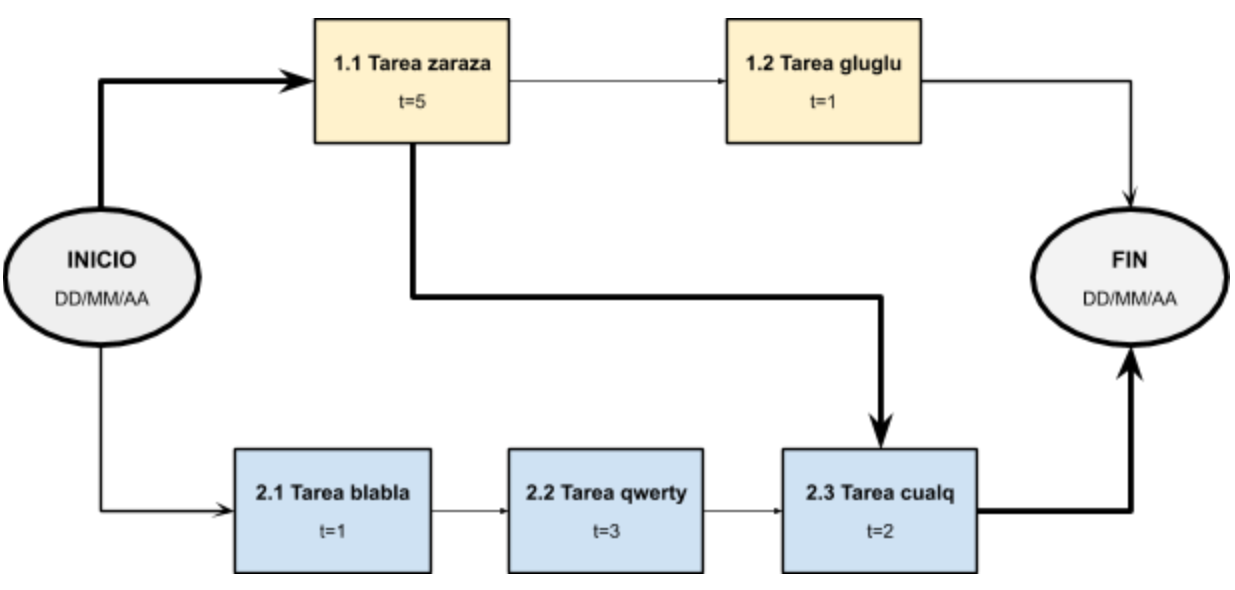
\includegraphics[width=1.0\textwidth]{./Figuras/AoN.png}
\caption{Diagrama en \textit{Activity on Node}}
\label{fig:AoN}
\end{figure}

\begin{figure}[H]
\centering 
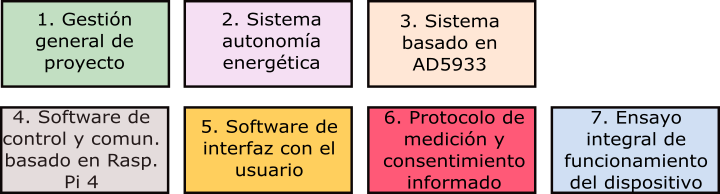
\includegraphics[width=.6\textwidth]{./Figuras/AoN_codigo.png}
\caption{Código de colores para cada grupo de tareas}
\label{fig:AoN_codigo}
\end{figure}

\pagebreak
\section{8. Diagrama de Gantt}
\label{sec:gantt}

\begin{consigna}{red}

\begin{figure}[H]
\centering 
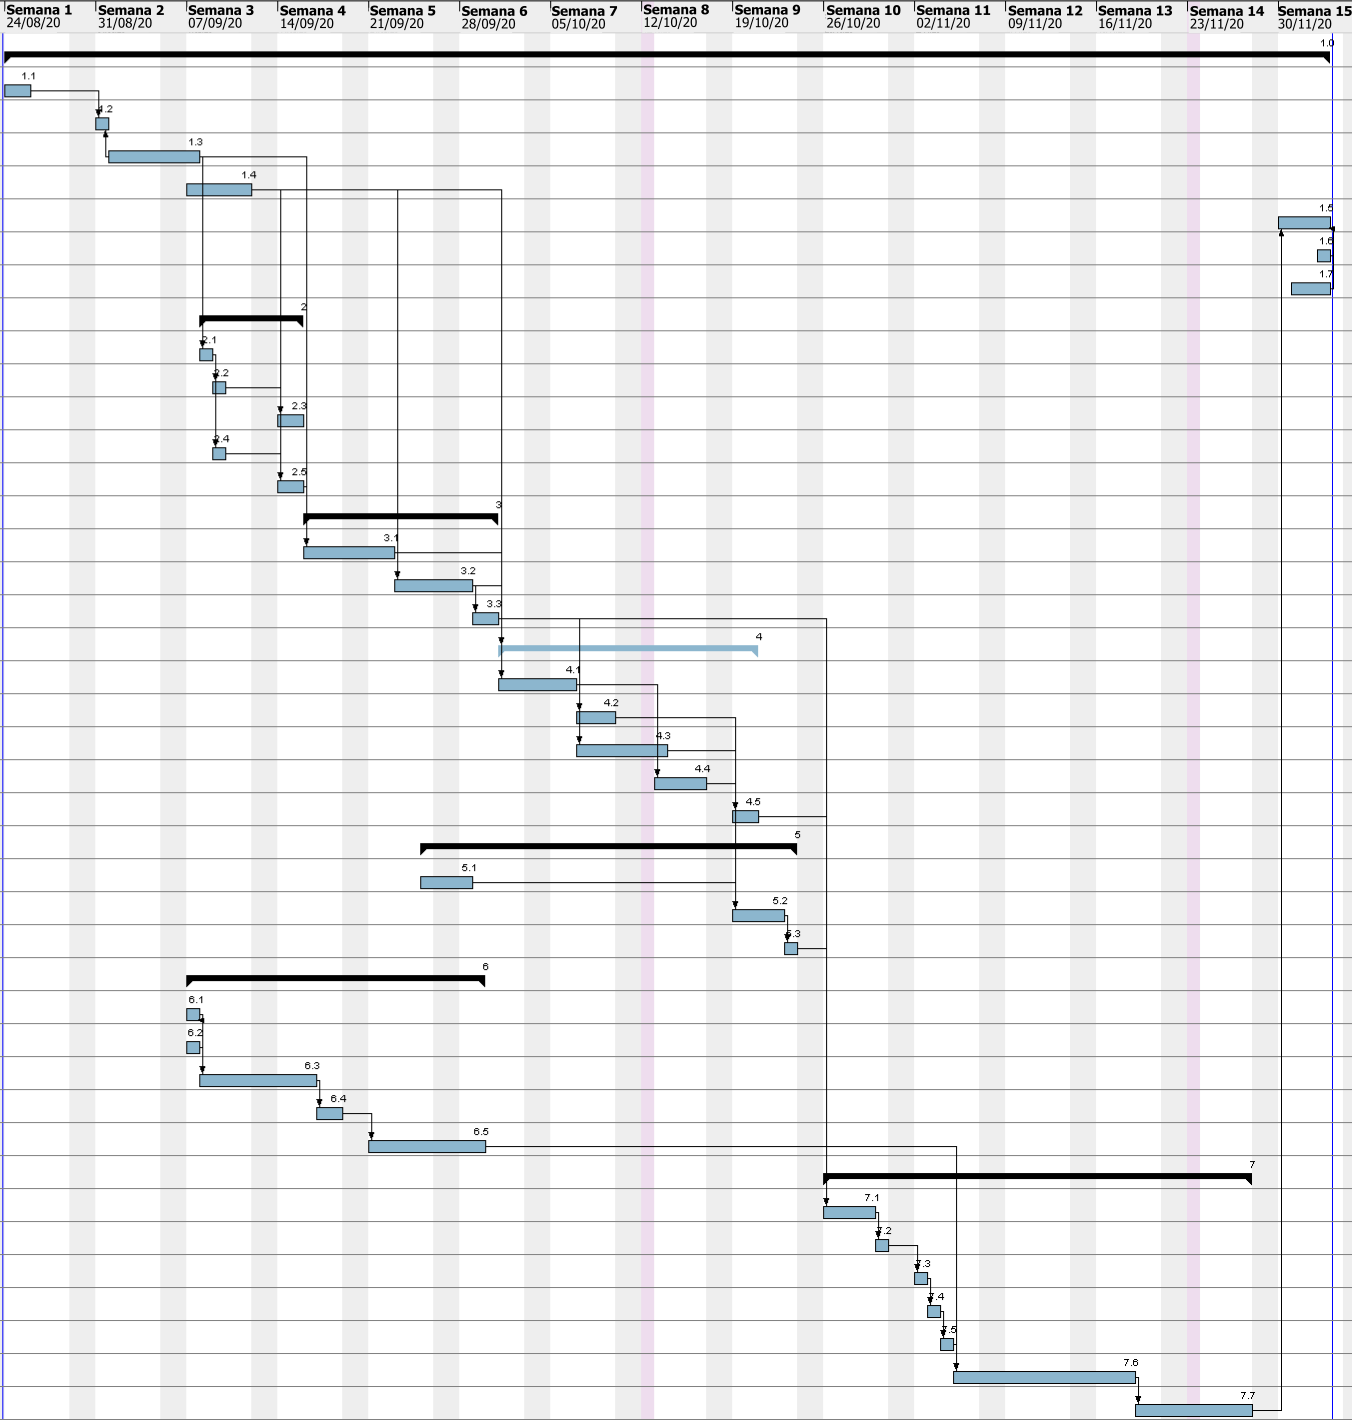
\includegraphics[width=1.0\textwidth]{./Figuras/gantt_final.png}
\caption{Diagrama de Gantt con las tareas descritas por su código}
\label{fig:gantt}
\end{figure}
\end{consigna}

\pagebreak
\section{9. Matriz de uso de recursos de materiales}
\label{sec:recursos}

\begin{table}[H]
\label{tab:recursos}
\centering
\begin{tabularx}{\linewidth}{@{}|c|X|X|X|X|X|X|@{}}
\hline
\cellcolor[HTML]{C0C0C0} & \cellcolor[HTML]{C0C0C0} & \multicolumn{5}{c|}{\cellcolor[HTML]{C0C0C0}Recursos requeridos (horas)} \\ \cline{3-6} 
\multirow{-2}{*}{\cellcolor[HTML]{C0C0C0}\begin{tabular}[c]{@{}c@{}}Código\\ WBS\end{tabular}} & \multirow{-2}{*}{\cellcolor[HTML]{C0C0C0}\begin{tabular}[c]{@{}c@{}}Nombre \\ tarea\end{tabular}} & Instrumental electrónico & Raspberry Pi4 & Sistema AD5933 & BioZmeter (*) & Copiadora \\ \hline
1.5 & Elaboración del manual de uso & 0  & 0 & 0  & 0 & 20 \\ \hline
1.7 & Escritura del informe final & 0 & 0 & 0  & 0 & 15 \\ \hline
2.2	& Diseño de circuito de carga & 8 & 8 & 0 & 0 & 0\\ \hline
2.3	& Implementa- ción de circuito de carga & 12 & 12  & 0  & 0 & 0 \\ \hline
2.4	& Diseño de circuito de regulación & 8 & 8 & 0 & 0 & 0\\ \hline
2.5	& Implementa- ción de circuito de regulación & 12 & 12  & 0  & 0 & 0 \\ \hline
3.1	& Diseño del sistema & 40 & 40 & 0  & 0  & 0\\ \hline
3.2	& Elaboración de la placa del circuito impreso & 30 & 0  & 0  &  0 & 0\\ \hline
3.3	& Ensamble y soldado de la placa del sistema y electrodos aplicables & 15 & 0 & 0   & 0 & 0\\ \hline
4.2 & Desarrollo del firmware de comunicación inalámbrica con dispositivo móvil & 0  & 25  & 25 & 0 & 0\\ \hline

\end{tabularx}%
\end{table}

\begin{table}[H]
\label{tab:recursos}
\centering
\begin{tabularx}{\linewidth}{@{}|c|X|X|X|X|X|X|@{}}
\hline
\cellcolor[HTML]{C0C0C0} & \cellcolor[HTML]{C0C0C0} & \multicolumn{5}{c|}{\cellcolor[HTML]{C0C0C0}Recursos requeridos (horas)} \\ \cline{3-6} 
\multirow{-2}{*}{\cellcolor[HTML]{C0C0C0}\begin{tabular}[c]{@{}c@{}}Código\\ WBS\end{tabular}} & \multirow{-2}{*}{\cellcolor[HTML]{C0C0C0}\begin{tabular}[c]{@{}c@{}}Nombre \\ tarea\end{tabular}} & Instrumental electrónico & Raspberry Pi4 & Sistema AD5933 & BioZmeter (*) & Copiadora \\ \hline
4.3	& Desarrollo del firmware de comunicación con sistema AD5933 &  0  & 20  & 20 & 0 & 0\\ \hline
4.4	& Desarrollo del firmware de control &  0  & 30  & 30 & 0 & 0\\ \hline
4.5	& Pruebas de funcionamiento  & 20  & 20 & 20 & 0 & 0 \\ \hline
5.2	& Desarrollo de software & 0 & 25 & 25 & 0 & 0 \\ \hline
5.3	& Pruebas de funcionamiento & 0 & 15 & 15  & 0 & 0 \\ \hline
7.2	& Mediciones sobre circuitos de componentes pasivos R-C & 2  & 2 & 2 & 2 & 0 \\ \hline
7.4	& Mediciones sobre sistemas biológicos ex-vivo & 3  & 3 & 3 & 3 & \\ \hline
7.6	& Mediciones sobre voluntarios humanos & 0 & 40 & 40  & 40 & 0\\ \hline

\end{tabularx}%
\end{table}

(*) BioZmeter: es la denominación del dispositivo desarrollado e integrado en la tarea 7.1.

\pagebreak
\section{10. Presupuesto detallado del proyecto}
\label{sec:presupuesto}

\begin{consigna}{black}
El presente proyecto se lleva adelante al interno del IDEI-UNTDF, los costos indirectos corren por cuenta de la institución siendo información que no está al alcance de un director de un proyecto de investigación y desarrollo, razón por la cual se detallan los costos pero no se colocan valores.
\end{consigna}

\begin{table}[htpb]
\centering
\begin{tabularx}{\linewidth}{@{}|X|c|r|r|@{}}
\hline
\rowcolor[HTML]{C0C0C0} 
\multicolumn{4}{|c|}{\cellcolor[HTML]{C0C0C0}COSTOS DIRECTOS} \\ \hline
\rowcolor[HTML]{C0C0C0} 
Descripción &
  \multicolumn{1}{c|}{\cellcolor[HTML]{C0C0C0}Cantidad} &
  \multicolumn{1}{c|}{\cellcolor[HTML]{C0C0C0}Valor unitario} &
  \multicolumn{1}{c|}{\cellcolor[HTML]{C0C0C0}Valor total} \\ \hline
 Raspberry Pi 4 4gb con Kit & 
  \multicolumn{1}{c|}{2} & 
  \multicolumn{1}{c|}{15629,00} & 
  \multicolumn{1}{c|}{31258,00} \\ \hline
Capacitores 885060 (kit de varios valores y cantidades) &
  \multicolumn{1}{c|}{1} & 
  \multicolumn{1}{c|}{14805,00} & 
  \multicolumn{1}{c|}{14805,00} \\ \hline
 Resistores KIT-RMCF0402FT-04 (kit de varios valores y cantidades) &
   \multicolumn{1}{c|}{1} & 
  \multicolumn{1}{c|}{3999,47} & 
  \multicolumn{1}{c|}{3999,47} \\ \hline
Diodos TPD2E001DRLRG4 &
   \multicolumn{1}{c|}{5} & 
  \multicolumn{1}{c|}{47,38} & 
  \multicolumn{1}{c|}{236,90} \\ \hline
Integrados MIC5319-3.3YD5-TR & 
  \multicolumn{1}{c|}{4} & 
  \multicolumn{1}{c|}{139,59} & 
  \multicolumn{1}{c|}{558,36} \\ \hline
Integrados AD5933 &
  \multicolumn{1}{c|}{4} & 
  \multicolumn{1}{c|}{4104,00} & 
  \multicolumn{1}{c|}{16416,00} \\ \hline
Integrado LTC1044ACS8 &
   \multicolumn{1}{c|}{4} & 
  \multicolumn{1}{c|}{618,64} & 
  \multicolumn{1}{c|}{2474,56} \\ \hline
kit Conectores 0766500009 &
   \multicolumn{1}{c|}{1} & 
  \multicolumn{1}{c|}{8441,61} & 
  \multicolumn{1}{c|}{8441,61} \\ \hline
Integrados OPA2376AIDGKR &
   \multicolumn{1}{c|}{5} & 
  \multicolumn{1}{c|}{221,02} & 
  \multicolumn{1}{c|}{1105,10} \\ \hline
Bateria  (modelo a definir) &
  \multicolumn{1}{c|}{2} & 
  \multicolumn{1}{c|}{5000,00} & 
  \multicolumn{1}{c|}{10000,00} \\ \hline
Latiguillos de electrocardiografía (set x5) &
  \multicolumn{1}{c|}{2} &
  \multicolumn{1}{c|}{1500,00} &
  \multicolumn{1}{c|}{3000,00} \\ \hline
Electrodos autoadhesivos/descartables de electrocardiografía (sobre x50) &
  \multicolumn{1}{c|}{2} &
  \multicolumn{1}{c|}{352,50} &
  \multicolumn{1}{c|}{705,00} \\ \hline
Cables pacientes para monitores multiparamétros con ficha DB15 &
  \multicolumn{1}{c|}{1} &
  \multicolumn{1}{c|}{7000,00} &
  \multicolumn{1}{c|}{7000,00} \\ \hline


\multicolumn{3}{|c|}{SUBTOTAL} &
  \multicolumn{1}{c|}{90000,00} \\ \hline
\rowcolor[HTML]{C0C0C0} 
\multicolumn{4}{|c|}{\cellcolor[HTML]{C0C0C0}COSTOS INDIRECTOS} \\ \hline
\rowcolor[HTML]{C0C0C0} 
Descripción &
  \multicolumn{1}{c|}{\cellcolor[HTML]{C0C0C0}Cantidad} &
  \multicolumn{1}{c|}{\cellcolor[HTML]{C0C0C0}Valor unitario} &
  \multicolumn{1}{c|}{\cellcolor[HTML]{C0C0C0}Valor total} \\ \hline

 Uso de Laboratorio y oficinas (Internet, Electricidad, Calefacción, etc.) &
  \multicolumn{1}{c|}{ - } &
  \multicolumn{1}{c|}{ - } &
  \multicolumn{1}{c|}{ - } \\ \hline
  
 Personal no docente administrativo (SCyT y Secretarias IDEI)  &
  \multicolumn{1}{c|}{ - } &
  \multicolumn{1}{c|}{ - } &
  \multicolumn{1}{c|}{ - } \\ \hline
  
 Personal no docente de legales (asesoramiento) &
  \multicolumn{1}{c|}{ - } &
  \multicolumn{1}{c|}{ - } &
  \multicolumn{1}{c|}{ - } \\ \hline
   
 Personal docente-investigador involucrado &
  \multicolumn{1}{c|}{ - } &
  \multicolumn{1}{c|}{ - } &
  \multicolumn{1}{c|}{ - } \\ \hline
  
\multicolumn{3}{|c|}{SUBTOTAL} &
  \multicolumn{1}{c|}{ - } \\ \hline
\rowcolor[HTML]{C0C0C0}
\multicolumn{3}{|c|}{TOTAL} & 90000,00
   \\ \hline
\end{tabularx}%
\end{table}

\pagebreak
\section{11. Matriz de asignación de responsabilidades}
\label{sec:responsabilidades}
\begin{consigna}{black}

\begin{table}[htpb]
\centering
\begin{turn}{270}
\resizebox{1.4\textwidth}{!}{%
\begin{tabular}{|c|c|c|c|c|c|c|c|c|}
\hline
\rowcolor[HTML]{C0C0C0} 
%\cellcolor[HTML]{C0C0C0} &
%  \cellcolor[HTML]{C0C0C0} &
%  \multicolumn{4}{c|}{\cellcolor[HTML]{C0C0C0}Listar todos los nombres y roles del proyecto} \\ \cline{3-6} 
\rowcolor[HTML]{C0C0C0} 
\cellcolor[HTML]{C0C0C0} &
  \cellcolor[HTML]{C0C0C0} &
  Responsable &
  Equipo &
  Equipo &
  Colaborador &
  Colaborador &
  Colaborador &
  Cliente \\ \cline{3-6} 
\rowcolor[HTML]{C0C0C0} 
\multirow{-2}{*}{\cellcolor[HTML]{C0C0C0}\begin{tabular}[c]{@{}c@{}}Código\\ WBS\end{tabular}} &
  \multirow{-3}{*}{\cellcolor[HTML]{C0C0C0}Nombre de la tarea} &
  Dell'Osa &
  Prisching &
  Dondo &
  Silva &
  Mailing &
  Masner &
  Santiago  \\ \hline
1  & \textbf{Gestión general de proyecto}   &  &  &  &  &  &  & \\ \hline
1.1 & Fase de Inicio del proyecto &	P  & S & C  &	C  & & &	A \\ \hline
1.2	& Definición de Alcance  &	P &	S &	C &	C &	C &	C &	A\\ \hline
1.3 & Estudio de la normativa IRAM 4220-1 &	S &	 &	P &	 &	C &	 &	 \\ \hline		
1.4 & Compras y adquisiciones &	P &	S  & & & & & \\ \hline
1.5 & Elaboración del manual de uso & P & &	S &	C &	C &	C &	 \\ \hline
1.6 & Rendición de compras y adquisiciones & P & S & & & & & A \\ \hline
1.7 & Escritura del informe final &	P &	C &	C & & C & &	 A \\ \hline
2 & \textbf{Sistema autonomía energética}   &  &  &  &  &  &  & \\ \hline
2.1 & Análisis y elección de batería &  &  & S &  & 	P &  & \\ \hline
2.2 & Diseño de circuito de carga &  &  & S &  & 	P &  & \\ \hline
2.3 & Implementación de circuito de carga & A & I & S &  & 	P &  & \\ \hline
2.4 & Diseño de circuito de regulación &  &  & P &  &	S &  & \\ \hline
2.5 & Implementación de circuito de regulación &  A & I & P &  & 	S &  & \\ \hline
3	 & \textbf{Sistema basado en AD5933}	&  &  &  &  &  &  & \\ \hline						
3.1	 & Diseño del sistema & A &  &	P & & S &  & \\ \hline
3.2	 & Elaboración de la placa del circuito impreso  & & & P & & S & & \\ \hline
3.3	 & Ensamble y soldado de la placa del sistema y electrodos aplicables &A &I &P &I & S &  & \\ \hline

								
4 & \textbf{Software de control y comunicación basado en Raspberry Pi 4} &  &  &  &  &  &  & \\ \hline				
4.1 & Diagramación de la arquitectura  & C & P & S & & C &  & \\ \hline
4.2 & Desarrollo del firmware de comunicación inalámbrica con dispositivo móvil &I &P & C	 & & & & \\ \hline
4.3 & Desarrollo del firmware de comunicación con sistema AD5933 & I & P & C & & C &  & \\ \hline		
4.4 & Desarrollo del firmware de control & C & P &	& &	S &  & \\ \hline
4.5 & Pruebas de funcionamiento & A & P & S & &	C &  & \\ \hline

5 & \textbf{Software de interfaz con el usuario} &  &  &  &  &  &  & \\ \hline	
5.1 & Diagramación de la interfaz (diseño y estructura)& A & P &	& C & &	C &	 \\ \hline
5.2	& Desarrollo de software &A & P & S & & & & \\ \hline								

5.3	& Pruebas de funcionamiento & A & P & S & C & & C & \\ \hline
6 & \textbf{Protocolo de medición y Consentimiento informado (CI)} &  &  &  &  &  &  & \\ \hline
6.1 & Escritura del Protocolo de Medición & I &  &  & P &  & S & \\ \hline
6.2 & Escritura del CI  & I &  &  & S &  & P & 	\\ \hline
6.3 & Primer Envío del protocolo y el CI a comité de bioética externos (CBE) para su revisión & P &  &  & C &  & S & A  \\ \hline
6.4 & Corrección del protocolo y CI a partir de la devolución del CBE & I &  &  & P & & S &	\\ \hline
6.5 & Segundo Envío del protocolo y el CI a CBE para su aprobación definitiva & P &  &  & C &  & S & A  \\ \hline
7 & \textbf{Ensayo integral de funcionamiento del dispositivo}	&  &  &  &  &  &  & \\ \hline						
7.1 & Implementación integral del dispositivo & A & S & P &  & C &  & 	\\ \hline
7.2 & Mediciones sobre circuitos de componentes pasivos R-C & P &  & S &  & C &  & 	\\ \hline	
7.3 & Análisis de mediciones en circuito R-C & P & I & S &  & C &  & \\ \hline		
7.4 & Mediciones sobre sistemas biológicos ex-vivo & P &  & S &  & 	C & C & \\ \hline
7.5 & Análisis de mediciones en sistemas biológicos ex-vivo & P & I & S &  & C & C & \\ \hline	
7.6 & Mediciones sobre voluntarios humanos & S  &  &  & P &  & 	A & \\ \hline
7.7 & Análisis de mediciones sobre seres humanos & S & I &  & P & C & A & I \\ \hline


 \end{tabular}%
}
\end{turn}
\end{table}

{\footnotesize
Referencias de la siguiente tabla:
\begin{itemize}
	\item P = Responsabilidad Primaria
	\item S = Responsabilidad Secundaria
	\item A = Aprobación
	\item I = Informado
	\item C = Consultado
\end{itemize}
} %footnotesize

%Una de las columnas debe ser para el Director, ya que se supone que participará en el proyecto.
%A su vez se debe cuidar que no queden muchas tareas seguidas sin ``A'' o ``I''.
%
%Importante: es redundante poner ``I/A'' o ``I/C'', porque para aprobarlo o responder %consultas primero la persona debe ser informada.

\end{consigna}

\pagebreak
\section{12. Gestión de riesgos}
\label{sec:riesgos}

\begin{consigna}{red}
Riesgo 1: Demora en la entrega del subsidio económico brindado por la SCyT-UNTDF.
\begin{itemize}
\item Severidad (S): 10 - Imposibilidad de comprar el material indispensable.
\item Ocurrencia (O): 7 - Inestabilidad económica del Estado Nacional repercute en las universidades nacionales.
\end{itemize}

Riesgo 2: Demoras e inconvenientes con procesos de compras y adquisiciones.
\begin{itemize}
\item Severidad (S): 10 - Imposibilidad de contar con los materiales indispensables.
\item Ocurrencia (O): 6 - Los proyectos de investigación suelen no ser una prioridad frente a necesidades de docencia y/o rescate económico de estudiantes.
\end{itemize}

Riesgo 3: Rotura del integrado AD5933  y Raspberry Pi por configuración eléctrica errónea o extravío.
\begin{itemize}
\item Severidad (S): 10 - Ambos componentes son las parte neurálgica del prototipo.
\item Ocurrencia (O): 5 - Los laboratorios de trabajo son compartidos con otros proyectos, usuarios y los estudiantes tienen acceso pseudo ilimitado.
\end{itemize}

Riesgo 4: Deserción de algún miembro del equipo o colaborador.
\begin{itemize}
\item Severidad (S): 8 - Cada interesado de estos grupos realiza tareas que otros miembro no realiza en su totalidad, la deserción de un miembro sobrecargaría de trabajo a dos o más de los otros miembros.
\item Ocurrencia (O): 3 - El compromiso asumido esta garantizado por experiencia de trabajos anteriores.
\end{itemize}

Riesgo 5: Inaccesibilidad a una institución de salud para tomar mediciones sobre pacientes fracturados.
\begin{itemize}
\item Severidad (S): 9 - No se alcanzaría la utilidad final del prototipo.
\item Ocurrencia (O): 5 - No es la prioridad de una institución de salud atender las pruebas de investigadores externos. Esta ponderación aumenta a 10 en épocas de pandemia. 
\end{itemize}


\begin{table}[H]
\centering
\begin{tabularx}{\linewidth}{@{}|X|c|c|c|c|c|c|@{}}
\hline
\rowcolor[HTML]{C0C0C0} 
Riesgo & S & O & RPN & S* & O* & RPN* \\ \hline
1.Demora en la entrega del subsidio económico brindado por la SCyT-UNTDF & 10 & 7 & 70 & 10 & 3 & 30 \\ \hline
2.Demoras e inconvenientes con procesos de compras y adquisiciones & 10 & 6 & 60 & 3 & 5 & 15 \\ \hline
3.Rotura del integrado AD5933  y Raspberry Pi por configuración eléctrica errónea & 10 & 5 & 50 & 5 & 3 & 15 \\ \hline
4.Deserción de algún miembro del equipo o colaborador & 8 & 3 & 24 &    &    &      \\ \hline
5.Inaccesibilidad a una institución de salud para tomar mediciones sobre pacientes fracturados & 9 & 5 & 45 & 4 & 3 & 12 \\ \hline
\end{tabularx}%
\end{table}

Criterio adoptado: 
Se tomarán medidas de mitigación en los riesgos cuyos números de RPN sean mayores a 40. Las escalas numéricas de Severidad y Ocurrencia son 1 a 10, aumentando el riesgo con el valor correspondiente.

Nota: los valores marcados con (*) en la tabla corresponden luego de haber aplicado la mitigación.

Plan de mitigación de los riesgos que originalmente excedían el RPN máximo establecido:
 
Riesgo 1: Demora en la entrega del subsidio económico brindado por la SCyT-UNTDF.
Mitigación: Búsqueda de ayudas económicas del Estado provincial y de donaciones en la industria electrónica fueguina.
\begin{itemize}
\item Severidad (S): 10 - Continua la imposibilidad de comprar el material indispensable en caso que el riesto se concrete.
\item Ocurrencia (O): 3 - En los últimos 3 años los proyectos a cargo de los mismos responsables se han llevado adelante mediante estos recursos financieros y materiales por la originalidad y el impacto social de los proyectos biomédicos localmente.
\end{itemize}

Riesgo 2: Demoras e inconvenientes con procesos de compras y adquisiciones.
Mitigación: Búsqueda de ayudas económicas del Estado provincial y de donaciones en la industria electrónica fueguina.
\begin{itemize}
\item Severidad (S): 3 - Las compras se realizan de forma directa sin la necesidad de trámites administrativos.
\item Ocurrencia (O): 5 - Posibilidad de inconvenientes a nivel de importaciones.
\end{itemize}

Riesgo 3: Rotura del integrado AD5933  y Raspberry Pi por configuración eléctrica errónea o extravío.
Mitigación: Adquisición de dos o más de cada uno de estos componentes alojados en lugares de acceso reservado para investigadores del proyecto.
\begin{itemize}
\item Severidad (S): 5 - En caso de rotura o extravío hay reemplazo.
\item Ocurrencia (O): 3 - Ante la posesión de reemplazos y alojamiento en lugares de dificil acceso baja la probabilidad.
\end{itemize}

Riesgo 5: Inaccesibilidad a una institución de salud para tomar mediciones sobre pacientes fracturados.
Mitigación: Incorporar a instituciones de salud externas al ámbito local, incluso internacional. El responsable del proyecto trabaja establemente con grupos de investigación médica de otras ciudades argentinas y extranjeras.
\begin{itemize}
\item Severidad (S): 4 - Enviar el prototipo vía postal y capacitar por medio de videoconferencias.
\item Ocurrencia (O): 3 - Estos grupos de investigación trabajan en instituciones de salud que son centros de investigación simultáneamente. Esta ponderación aumenta a 10 en épocas de pandemia. 
\end{itemize}

\end{consigna}


\section{13. Gestión de la calidad}
\label{sec:calidad}

\begin{consigna}{red}

VERIFICAR QUE SIEMPRE QUE HABLO DEL DESARROLLO SEA "PROTOTIPO" Y CUANDO HABLO DE CELULAR/PC/TABLET SEA "DISPOSITIVOS"


\begin{enumerate}
\item Grupo de requerimientos asociados con la normativa vigente
	\begin{enumerate}
	\item Se debe cumplir con la normativa IRAM 4220-1 (Seguridad eléctrica de equipamiento médico)
	\begin{itemize}
		\item Verificación: Medir de corrientes aplicadas por electrodos aplicables y corrientes de fugas por carcaza.\\
		\item Validación: Certificado de Laboratorio de Metrología\\
	\end{itemize}
	\item Se debe cumplir con la normativa de principios éticos para las investigaciones médicas en seres humanos
	\begin{itemize}
		\item Verificación: Verificar el cumplimiento del escrito elaborado con lo estipulado en la declaración de Helsinki del año 2000.\\
		\item Validación: Acta de aprobación de comité de bioética.\\
	\end{itemize}
	\end{enumerate}

\item Grupo de requerimientos asociados con adquisición de datos
	\begin{enumerate}
	\item Se debe contar con tres pares de electrodos aplicables de forma no invasiva para configuración de electrodos bipolar y selección por interruptor manual.
	\begin{itemize}
		\item Verificación: Contar la cantidad de electrodos y medir cada par de ellos son fantomas eléctricos. \\
		\item Validación: Demostración sobre fantomas seleccionando desde la interfaz de usuario cada uno de los tres pares de electrodos.\\
	\end{itemize}	
	\item Se debe poseer una resolución de la medición en orden de los 10 ohmios.
	\begin{itemize}
		\item Verificación: Tomar mediciones sobre fantomas eléctricos con resistencias variables de alta precisión en los rangos de la precisión necesaria y comparación con simulaciones computacionales. \\
		\item Validación: Certificado de Laboratorio de Metrología.\\
	\end{itemize}
	\item No se debe configurar el rango de frecuencias de señales aplicables (será fijo entre 5kHz y 100kHz).
	\begin{itemize}
		\item Verificación: Realizar mediciones con espectroscopio.\\
		\item Validación: Demostración de una medida estándar sobre fantoma y nuestra de resultado en forma gráfica en el dominio de la frecuencia.\\
	\end{itemize}
	\end{enumerate}
\item Grupo de requerimientos asociados con la interfaz con el usuario
	\begin{enumerate}
	\item Se debe contar con la visualización del módulo de la bioimpedancia en el dominio de la frecuencia en gráfico XY.
	\item Se debe contar con la visualización de los valores numéricos de módulo de bioimpedancia para cada frecuencia.
\begin{itemize}
		\item Verificación: Realizar un inspección visual de la interfaz del usuario en la visualización de resultados y la correcta realización del gráfico XY con el dominio en los valores de frecuencia y la imagen en los valores del módulo de impedancia.\\
		\item Validación: Visualización de los resultados obtenidos en ambos formatos (gráfica y tabla de valores) a partir de la prueba de demostración con un fantoma.\\
\end{itemize}	
	\item Se debe poder descargar de los datos medidos en un archivo formato .CSV (o similar) en una memoria extraíble (tipo microSD).
	\begin{itemize}
		\item Verificación: Realizar inspección de la generación de archivo con datos separados por comas y de la correcta grabación en memoria extraíble.\\
		\item Validación: Descarga de los datos y posterior lectura con memoria extraíble con correcta apertura del archivo generado.\\
	\end{itemize}
\end{enumerate}

\item Grupo de requerimientos asociados con portabilidad
	\begin{enumerate}
	\item Se debe contar con una autonomía a baterías de al menos 2 horas y conector USB para la carga de la bateria.
	\begin{itemize}
		\item Verificación: Calcular de consumo estimativo de Raspberry y componentes electrónicos principales a partir de sus hojas de datos.\\
		\item Validación: Prueba de autonomía del prototipo en uso durante dos horas.\\
	\end{itemize}
	\item No se deben exceder las dimensiones físicas externas de 15 centímetros de largo, 8 centímetros de ancho y 3 centímetros de espesor.
	\begin{itemize}
		\item Verificación: Realizar mediciones de las dimensionales en escala de centímetros.\\
		\item Validación: Mostrar resultados de las mediciones dimensionales.\\
	\end{itemize}
	\item Se debe contar con la disipación térmica conveniente para que la carcasa externa no genere una temperatura perceptible por el usuario.
	\begin{itemize}
		\item Verificación: Realizar mediciones térmicas a carcaza cerrada en durante el funcionamiento continuo del dispositivo.\\
		\item Validación: Mostrar resultados de las mediciones térmicas.\\
	\end{itemize}
	\item Se debe contar con conectividad inálambrica (wifi y/o Bluetooth) a un dispositivo smartphone, tablet o PC-notebook.
	\begin{itemize}
		\item Verificación: Inspección del correcto funcionamiento de conectividad en cada uno de los dispositivos detallados.\\
		\item Validación: Demostración de la prestación en smartphone, tablet o PC-notebook\\
	\end{itemize}
	\end{enumerate}
	
\end{enumerate}

\end{consigna}

\section{14. Comunicación del proyecto}
\label{sec:comunicaciones}

\begin{consigna}{red}
El plan de comunicación del proyecto es el siguiente:
\end{consigna}

% Please add the following required packages to your document preamble:
% \usepackage{graphicx}
% \usepackage[table,xcdraw]{xcolor}
% If you use beamer only pass "xcolor=table" option, i.e. \documentclass[xcolor=table]{beamer}
\begin{table}[htpb]
\centering
\resizebox{\textwidth}{!}{%
\begin{tabular}{|c|c|c|c|c|c|}
\hline
\rowcolor[HTML]{C0C0C0} 
\multicolumn{6}{|c|}{\cellcolor[HTML]{C0C0C0}PLAN DE COMUNICACIÓN DEL PROYECTO}           \\ \hline
\rowcolor[HTML]{C0C0C0} 
¿Qué comunicar? & Audiencia & Propósito & Frecuencia & Método de comunicac. & Responsable \\ \hline
                &           &           &            &                      &             \\ \hline
                &           &           &            &                      &             \\ \hline
                &           &           &            &                      &             \\ \hline
                &           &           &            &                      &             \\ \hline
                &           &           &            &                      &             \\ \hline
\end{tabular}%
}
\end{table}

\section{15. Gestión de Compras}
\label{sec:compras}

\begin{consigna}{red}
En caso de tener que comprar elementos o contratar servicios:
a) Explique con qué criterios elegiría a un proveedor.
b) Redacte el Statement of Work correspondiente.
\end{consigna}

\section{16. Seguimiento y control}
\label{sec:seguimiento}

\begin{consigna}{red}
Para cada tarea del proyecto establecer la frecuencia y los indicadores con los se seguirá su avance y quién será el responsable de hacer dicho seguimiento y a quién debe comunicarse la situación (en concordancia con el Plan de Comunicación del proyecto).

El indicador de avance tiene que ser algo medible, mejor incluso si se puede medir en \% de avance. Por ejemplo,se pueden indicar en esta columna cosas como ``cantidad de conexiones ruteadeas'' o ``cantidad de funciones implementadas'', pero no algo genérico y ambiguo como ``\%'', porque el lector no sabe porcentaje de qué cosa.

\end{consigna}

\begin{table}[!htpb]
\centering
\begin{tabularx}{\linewidth}{@{}|X|X|X|X|X|X|@{}}
\hline
\rowcolor[HTML]{C0C0C0} 
\multicolumn{6}{|c|}{\cellcolor[HTML]{C0C0C0}SEGUIMIENTO DE AVANCE}                                                                       \\ \hline
\rowcolor[HTML]{C0C0C0} 
Tarea del WBS & Indicador de avance & Frecuencia de reporte & Resp. de seguimiento & Persona a ser informada & Método de comunic. \\ \hline
 &  &  &  &  &  \\ \hline
 &  &  &  &  &  \\ \hline
 &  &  &  &  &  \\ \hline
 &  &  &  &  &  \\ \hline
 &  &  &  &  &  \\ \hline
\end{tabularx}%
%}
\end{table}

\section{17. Procesos de cierre}    
\label{sec:cierre}

\begin{consigna}{red}
Establecer las pautas de trabajo para realizar una reunión final de evaluación del proyecto, tal que contemple las siguientes actividades:

\begin{itemize}
\item Pautas de trabajo que se seguirán para analizar si se respetó el Plan de Proyecto original:
 - Indicar quién se ocupará de hacer esto y cuál será el procedimiento a aplicar. 
\item Identificación de las técnicas y procedimientos útiles e inútiles que se utilizaron, y los problemas que surgieron y cómo se solucionaron:
 - Indicar quién se ocupará de hacer esto y cuál será el procedimiento para dejar registro.
\item Indicar quién organizará el acto de agradecimiento a todos los interesados, y en especial al equipo de trabajo y colaboradores:
  - Indicar esto y quién financiará los gastos correspondientes.
\end{itemize}

\end{consigna}


\end{document}